\chapter{Producto}
\label{producto}


\section{Orquestación}

Un sistema de análisis a gran escala necesita coordinar y gestionar de manera robusta y confiable los procesos del flujo de trabajo, a esto se le llama orquestación. Existen varios orquestadores, tales como \texttt{Oozie, Azkaban y Luigi}. Para este proyecto se eligió  \href{http://luigi.readthedocs.org/en/stable/}{\texttt{luigi}}, que fue desarrollado por Spotify en el lenguaje \texttt{Python}. Este esquema tiene varias ventajas sobre los scripts simples, algunas de las cuales se enumeran a continuación:

\begin{enumerate}
\item \textbf{Modularidad}: El código se segmenta en pasos definidos, lo que facilita su mantenimiento y expansión.
\item \textbf{Robustez}: Se requiere que todos los pasos serializen sus resultados a disco, lo que hace que el sistema sea resistente a fallas y que no tenga que repetir todo el proceso después de un error.
\item \textbf{Idempotencia}: Si se programa correctamente, los procesos sólo corren una vez. Incluso si se corre el proceso una segunda vez, sólo corre lo que no haya sido corrido antes.
\item \textbf{Paralelismo}: Es bastante sencillo paralelizar los procesos que convenga para utilizar los núcleos de un servidor grande de manera eficiente.
\end{enumerate}



 \texttt{Luigi} ofrece estas ventajas, lo único que se requiere es que los pasos tengan entradas y salidas bien definidas; un proceso únicamente requiere sus dependencias para correr y debe arrojar los resultados que necesite la siguiente sección.

\texttt{Luigi} corre nativamente en \texttt{Python}, por lo que se puede hacer cualquier cosa que se pueda hacer en \texttt{Python}. Esto incluye llamar códigos en \texttt{shell}, \texttt{R} y muchos otros lenguajes. La mayoría de los procesos se hicieron directamente en \texttt{Python} por simplicidad, pero algunos se dejaron en otros lenguajes por su facilidad de uso.

A continuación se describe a grandes rasgos los pasos que componen el  \emph{pipeline} o diagrama de flujo. Cabe mencionar que esta es una descripción didáctica del proceso. Internamente hay algunos procesos que se efectúan en un orden ligeramente distinto al aquí presentado, por cuestiones computacionales.

 A continuación se muestra el diagrama de flujo de todo el proyecto, representado en la figura \ref{flujo}, las partes en verde son las correspondientes a los algoritmos  del ITAM, las figuras en blanco son los procesos desarrollados por el equipo de la UNAM/GIL.

\begin{figure}[H]
\centering
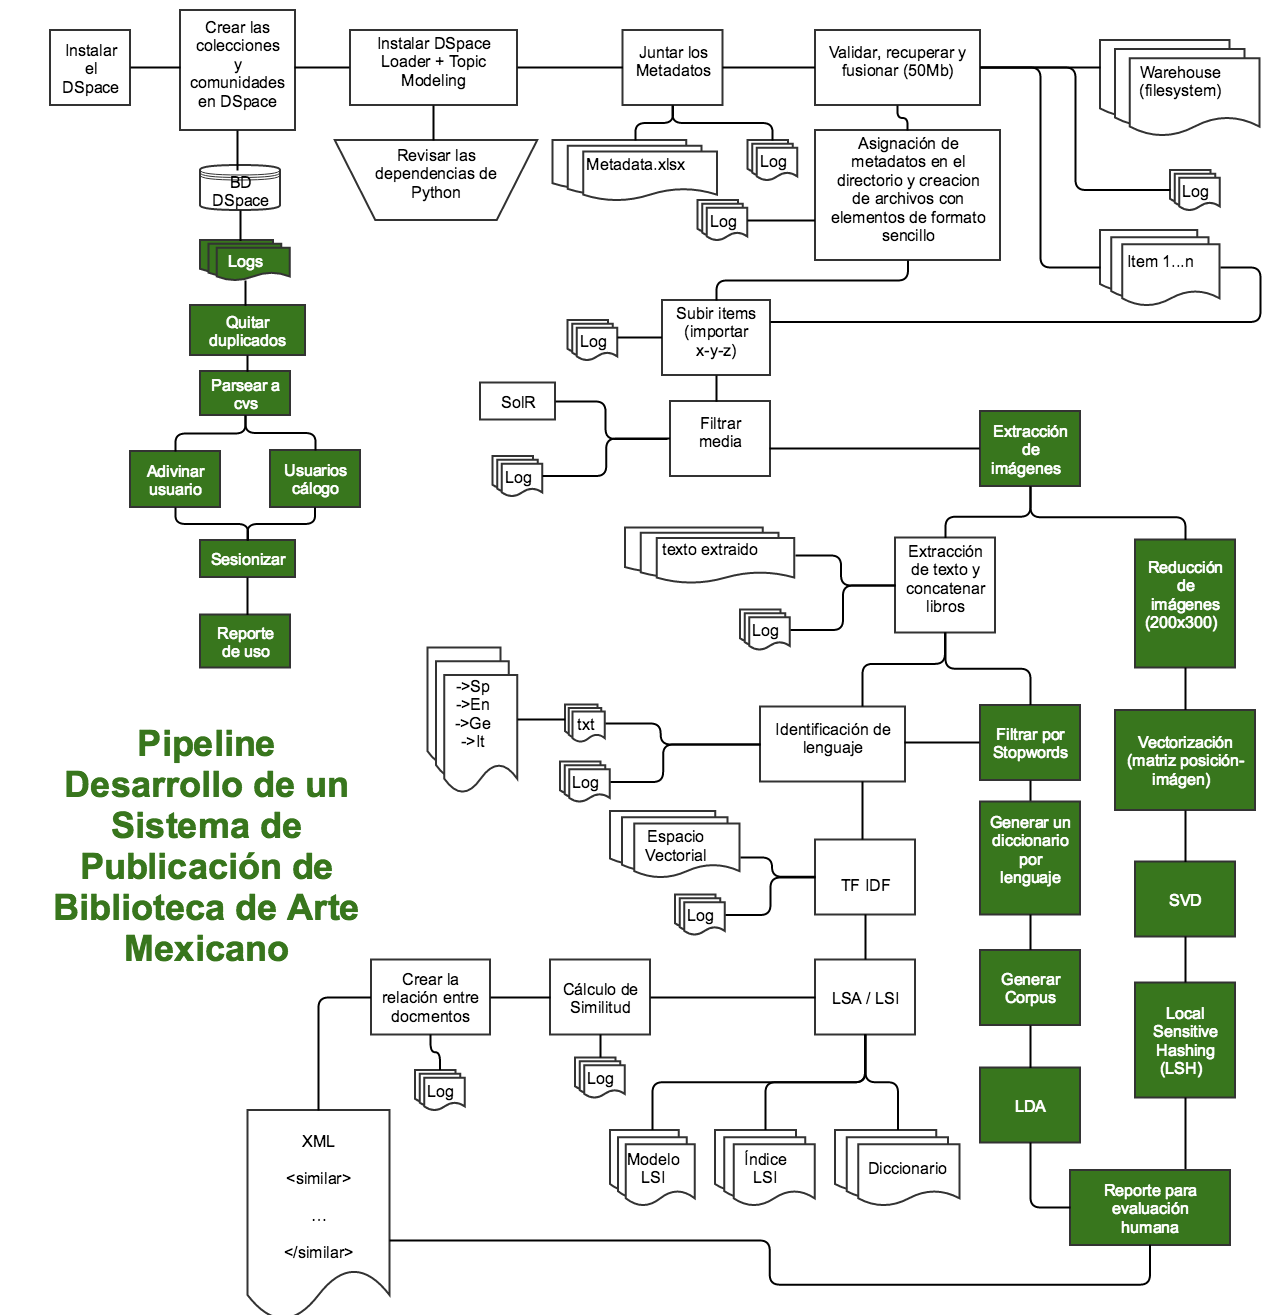
\includegraphics[width=1\textwidth]{Figures/pipeline.png}
\caption{Diagrama de flujo del proyecto}
\label{flujo}
\end{figure}

A continuación se describen  los pasos representados en el diagrama de flujo, desde los archivos en PDF crudos hasta las salidas necesarias para mostrar en el producto final. Cada proceso se detalla a profundidad en los tres capítulos subsecuentes.  

\subsection{Procesamiento de Texto} 
\subsubsection{ Extracción de texto}

\textbf{ Pegado de PDFs en archivos de 50 MB}

\begin{itemize}
\item \textbf{Input}: PDFs crudos, en el formato descrito abajo.
\item \textbf{Output}: Libros en formato PDF divididos en un conjunto de PDFs de hasta 50 MB.
\item \textbf{Paquetes relevantes}: \texttt{PyPDF2}
\end{itemize}

El pegado de PDFs empieza con una carpeta general en la que se encuentran todos los PDFs con respecto a la estructura de carpetas que se describe a continuación. Adentro de la carpeta de PDFs que contiene todos los libros debe haber una segunda carpeta por cada libro que respectivamente contenga los PDFs de las diversas hojas, por ejemplo: \texttt{pdf/libro\_de\_arte\_x/hoja\_i.pdf}

Con esta estructura se genera una segunda carpeta de PDFs general que contiene los libros pero en sub-PDFs de hasta 50 MB. En el ejemplo del libro: \textbf{libro\_de\_arte\_x}, se genera la salida:

\texttt{pdf\_full/libro\_de\_arte\_x/libro\_de\_arte\_x1deN.pdf}

\texttt{pdf\_full/libro\_de\_arte\_x/libro\_de\_arte\_x2deN.pdf}

$\vdots$

\texttt{pdf\_full/libro\_de\_arte\_x/libro\_de\_arte\_xNdeN.pdf},

en donde $N$ se refiere a la cantidad de archivos que se generan en total de forma que cada uno de los archivos que contienen el compilado de páginas sea menor de 50 MB.

Este proceso comienza generando una lista que describe el contenido de un libro completo, en donde cada entrada de la lista se refiere a una página y su respectivo tamaño en memoria. Con esta lista se utiliza el paquete de   \texttt{PyPDF2} de \texttt{Python} y se juntan recursivamente las páginas en nuevos PDFs de hasta 50 MB donde el nombre del pedazo del libro de hasta 50 MB se llama igual que el libro más un índice que sigue la metodología propuesta por la UNAM y como se describió en el ejemplo.

\textbf{Notas}
\begin{enumerate}
\item La estructura de las carpetas juega un papel fundamental en el proceso.
\item La carpeta de salida que contiene los PDFs de hasta 50 MB sigue la misma estructura de carpetas que se describió. 
De forma que la ruta de salida está al mismo nivel que la carpeta que contiene los PDFs originales, en este caso, la carpeta de salida  se llamó \texttt{pdf\_full$/$}, pero se puede modificar al gusto.
\item Cada archivo compilado de hasta 50 MB contiene distinto número de páginas ya que esto depende del espacio en memoria de las páginas individuales. 
\end{enumerate}

\textbf{Extracción de texto
a partir de PDFs y detección de idioma}

\begin{itemize}
\item \textbf{Input}: PDFs crudos, en el formato descrito abajo.
\item \textbf{Output}: Libros en formato texto tal cual fue extraído, archivos JSON con extractos de los libros.
\item \textbf{Paquetes relevantes}: \texttt{pdfminer}, \texttt{nltk}
\end{itemize}




El proceso empieza con una carpeta general en la que deben estar todos los PDFs. Adentro de ella debe haber una carpeta por libro que contenga los PDFs de las diversas hojas, por ejemplo: \texttt{pdf/libro\_de\_arte/hoja\_i.pdf}

Se extraen los textos utilizando el paquete  \texttt{pdfminer} de \texttt{Python} y se juntan los resultados de todas las hojas en un solo archivo por libro. Posteriormente se detecta el idioma de cada texto utilizando la metodología propuesta por la UNAM, la idea general es observar qué porcentaje de las \emph{stopwords} de cada idioma tiene un texto y se le asigna el idioma del que tenga mayor porcentaje. Después de la detección, los libros en versión texto se meten en una carpeta según su idioma. Adicionalmente, se guardan dos archivos de metadatos, uno con los idiomas registrados y otro con una relación entre los libros y sus idiomas correspondientes.

Por practicidad se optó por extraer los párrafos representativos en este mismo proceso. Para ello se tomaron 3 secciones de aproximadamente 500 letras al 10\%, 50\% y 90\% de avance del libro aproximadamente. El criterio tiene cierta flexibilidad e intenta encontrar párrafos completos (que empiecen en salto de línea y mayúscula), aunque esto en general es poco preciso por la imperfección del OCR efectuado al momento de digitalizar los libros.

\textbf{Notas}
\begin{enumerate}
\item Esta extracción se considera que tiene nivel de limpieza "nulo", por lo que los resultados de la extracción se meten a la carpeta `raw` dentro de la carpeta de textos.
\item Por razones internas del funcionamiento de \texttt{luigi}, es imposible revisar de antemano a qué carpeta debe ir cada libro, ya que no se puede saber su idioma antes de procesarlo. Para darle la vuelta a esta limitación, se generó una carpeta con un archivo de metadatos por libro, `libro.meta`, que sirve para que \texttt{luigi} pueda revisar el árbol de dependencias.
\end{enumerate}


\subsubsection{Limpieza de textos}

\begin{itemize}
\item \textbf{Input}: Libros en formato texto crudo.
\item \textbf{Parámetros}: Idioma(s) a procesar, nivel(es) de limpieza a obtener.
\item \textbf{Output}:Libros en formato texto limpio, según la especificación.
\item \textbf{Paquetes relevantes}: \texttt{nltk}, \texttt{unicodedata}
\end{itemize}


Según el nivel de limpieza elegido, se genera una estructura similar a la de los textos crudos (\emph{raw}. Los dos niveles son incrementalmente más "limpios":
\begin{itemize}
\item Limpieza básica (\emph{clean}):
    \begin{itemize}
   \item Se quitan los acentos.
   \item Se quitan los saltos de página.
    \item Se pasa todo a minúsculas.
    \item  Se quitan los caracteres especiales que queden después de quitar los acentos.
    \item  Se quitan palabras cortas (de 3 o menos caracteres).
    \item Se quitan palabras con algún carácter repetido 3 o más veces.
    \end{itemize}
\item Limpieza avanzada (\emph{stopwords}):
    \begin{itemize}
   \item  Se quitan las palabras poco informativas (\emph{stopwords}).
    \end{itemize}
\end{itemize}

Los dos pasos anteriores se generan de manera incremental, lo que significa que si se genera uno más avanzado, siempre se generan todos los anteriores. Cada nivel de limpieza genera una estructura similar a la generada en el paso de extracción (i.e. a la carpeta \emph{raw}), pero con nombre y características según sea el caso.

\textbf{Nota}: Nuevamente se utilizó un esquema de dependencias artificiales como en la extracción.

\subsubsection{ Minería de textos}

Una vez habiendo extraído y preparado los textos se puede empezar el proceso de minería. De aquí en adelante los procesos generan varios resultados, uno para cada nivel de limpieza y para cada idioma que se pida al comenzar el programa.

 \textbf{Vectorización de textos}


\begin{itemize}
\item \textbf{Input}: Textos de un idioma dado, con un nivel de limpieza dado.

\item \textbf{Output}:Un diccionario con los conteos de palabras y el corpus vectorizado (matriz términos - documentos).
\item \textbf{Paquetes relevantes}: \texttt{gensim}
\end{itemize}

Los algoritmos de minería necesitan entradas numéricas  que residen en espacios vectoriales. Por ello el primer paso del análisis es vectorizar los textos. En el paquete  \texttt{gensim} este proceso se divide en dos etapas: (1) generar un \emph{diccionario} con las palabras válidas dentro de la colección, y (2) generar una matriz términos - documentos, que contiene los conteos de cada término en cada documento. En  \texttt{gensim} se le llama \emph{corpus} a la matriz términos - documentos.

\subsubsection{ Latent Dirichlet Analysis (LDA): Clusters por tópicos}

\begin{itemize}

\item \textbf{Input}: Un diccionario con los conteos de palabras y el corpus vectorizado (matriz términos - documentos).
\item \textbf{Parámetros}: Número de tópicos a utilizar.
\item \textbf{Output}:Modelos LDA entrenados con los datos dados. Listas de tópicos y listas de libros asignadas a un conjunto (tópico a definir por experto), en diversos formatos (JSON, HTML, XML).
\item \textbf{Paquetes relevantes}: \texttt{gensim, pandas, pandoc, markdown}, \texttt{unicodedata}
\end{itemize}


El modelo LDA consiste en varias etapas:
\begin{enumerate}
\item Se entrenan varios modelos de LDA con base en los parámetros seleccionados por el usuario.
\item Cada modelo generado en el paso anterior predice o asigna una categoría, cluster o en este caso un tópico a cada libro de la colección.
\item  Se crean listas para poder consultar los resultados de la asignación de tópicos a los libros de la colección con cada modelo creado.
\end{enumerate}

Al finalizar los procesos mencionados se crean las carpetas `models` y `results` en las que se guardan los modelos de LDA y los resultados de los tópicos para la colección por cada modelo generado respectivamente. La visualización de los resultados está disponible en distintos formatos. Por ejemplo, el HTML permite explorar la asignación de los tópicos a los libros de la colección bajo distintos modelos y esto permite que un experto lo explore y elija los parámetros óptimos del modelo. El JSON permite explorar la información en otros sistemas. El XML permite interactuar interactuar con otros productos de forma simple. En este caso será el paquete DSpace en una página web.

El formato del XML es el siguiente:

\begin{lstlisting}
<?xml version="1.0" encoding="UTF-8"?>

<topicos>
		<topico numero="1" palabras="palabra_1, palabra_2, palabra_3 palabra_4, palabra_5">
			<libro>
					<titulo> libro_j </titulo>
					<probabilidad> proba_libro_j </probabilidad>
			</libro>
			<libro>
					<titulo> libro_k </titulo>
					<probabilidad> proba_libro_k </probabilidad>
			</libro>
		</topico>
		<topico numero="2" palabras='palabra_1, palabra_2, palabra_3 palabra_4, palabra_5'>
			<libro>
					<titulo> libro_i </titulo>
					<probabilidad> proba_libro_j </probabilidad>
			</libro>
			<libro>
					<titulo> libro_m </titulo>
					<probabilidad> proba_libro_m </probabilidad>
			</libro>
		</topico>
</topicos>
\end{lstlisting}

En donde se listan los tópicos por número y por las palabras que definen el respectivo tópico. Para cada tópico se incluye el título del libro junto con la probabilidad de pertenencia al respectivo tópico.


\subsubsection{ Latent Semantic Indexing (LSI): Documentos similares}

\begin{itemize}
\item \textbf{Input}: Un diccionario y un corpus.

\item \textbf{Parámetros}:Número de dimensiones latentes a utilizar.

\item \textbf{Output}: Modelo vectorizado transformado con TF-IDF. Listas los libros similares a cada libro, en diversos formatos (JSON, CSV, HTML, XML, red).

\item \textbf{Paquetes relevantes}: \texttt{gensim, pandas, markdown, pandoc}
\end{itemize}

El Análisis de Semántica Latente o LSI se lleva a cabo en varias etapas:
\begin{enumerate}

\item Se pondera el corpus con el modelo TF-IDF para \item  Se genera el modelo de semántica latente.
\item  Se calculan las similitudes entre los documentos y se guardan las más relevantes.

\end{enumerate}

Al finalizar estos procesos se tiene varios archivos con información de los modelos de  \texttt{gensim} y las salidas en diversos formatos. Cada uno de ellos tiene un fin distinto. Por ejemplo, el HTML y la red permiten visualizar fácilmente los resultados, con el fin de que un experto elija los parámetros óptimos del modelo, mientras que el JSON y el CSV permiten explotar la información en otros sistemas. El XML sirve para mostrar los resultados en la página web del producto. El formato del XML fue diseñado para atender las necesidades del equipo de la UNAM (GIL).

La estructura del XML es la siguiente:

\begin{lstlisting}
<?xml version="1.0" encoding="UTF-8"?>
<similitud>
	<libro handle="pdf/libro_1">
		<similar>
			<titulo>libro_1</titulo>
			<ranking>0</ranking>
			<sim>1.000000</sim>
		</similar>
		<similar>
			<titulo>libro_j</titulo>
			<ranking>1</ranking>
			<sim>similitud_libro_1_j</sim>
		</similar>
		<similar>
			<titulo>libro_k</titulo>
			<ranking>2</ranking>
			<sim>similitud_libro_1_k</sim>
		</similar>
	</libro>
	
	<libro handle="pdf/libro_2">
		<similar>
			<titulo>libro_2</titulo>
			<ranking>0</ranking>
			<sim>1.000000</sim>
		</similar>
		<similar>
			<titulo>libro_i</titulo>
			<ranking>1</ranking>
			<sim>similitud_libro_2_i</sim>
		</similar>
		<similar>
			<titulo>libro_m</titulo>
			<ranking>2</ranking>
			<sim>similitud_libro_2_m</sim>
		</similar>
	</libro>
\end{lstlisting}

En donde \texttt{handle} se refiere a la ruta donde se encuentra el libro $X$ respectivamente, en este caso,  \texttt{pdf/libro\_1}, y \texttt{similitud\_libro\_1\_j} se refiere a la similitud que tienen el libro 1 con el libro $j$. 

\textbf{Nota}: El algoritmo de LSI lo realizó el equipo de la UNAM, nosotros lo integramos en el flujo del proyecto por ser parte  complementaria del procesamiento en TF-IDF. 

\subsubsection{Procesamiento de Imágenes}

\subsubsection{ Identificación de imágenes}

Para identificar las imágenes de las páginas escaneadas se optó por hacer un conteo de los  colores que componen cada  página. A partir de este conteo de definió un rango para identificar las páginas que contienen imágenes, la idea detrás de este proceso es que las páginas con  imágenes contienen más colores que aquellas que solamente contienen texto. 



\begin{itemize}
\item \textbf{Input}: Archivos jpg.
\item \textbf{Output}: Listado csv por cada libro de aquellas páginas que su conteo de colores estuvo por arriba del rango.
\item \textbf{Paquetes relevantes}: \texttt{skimage}
\end{itemize}



\subsubsection{ Reducción y copiado de imágenes}

Una vez identificadas las páginas con imágenes, se copia estas imágenes  en una carpeta aparte y se reduce su tamaño a una escala de  200 x 300 píxeles  para homogeneizar la colección de imágenes. 

\begin{itemize}
\item \textbf{Input}: Archivos jpg con imágenes, listado de imágenes en csv.
\item \textbf{Output}: Imágenes reducidas.
\item \textbf{Paquetes relevantes}: \texttt{imagemagick}
\end{itemize}
 
\subsubsection{ Creación de matriz conteo de colores}

Para poder encontrar similitud, cada imagen debe ser vectorizada. Para hacer más eficiente el proceso el universo de colores se limitó a 1331 colores. Una vez creado el  vector del conteo para cada color  se  agrega a una matriz que concentra toda esta información.

\begin{itemize}
\item \textbf{Input}: Archivos jpg reducidos.
\item \textbf{Output}: Archivo csv con conteo de colores.
\item \textbf{Paquetes relevantes}: \texttt{dplyr}
\end{itemize}

\subsubsection{ Local Sensitive Hashing (LSH)}
Una vez que tenemos la matriz, se implementa el algoritmo de Local Sensitive Hashing (LSH) para encontrar las imágenes con mayor parecido, este es un proceso rápido y efectivo para encontrar similitudes en situaciones en las que hacer comparaciones de documento por documento es muy tardado.

\begin{itemize}
\item \textbf{Input}: Archivo csv con conteo de colores.
\item \textbf{Output}: Listado xml donde la primera columna representa un documento y la segunda el documento al que tiene un alto grado de similitud.
\item \textbf{Paquetes relevantes}: \texttt{dplyr}
\end{itemize}




\subsection{Procesamiento de clickstream}

Para obtener información sobre el uso del DSpace  se propone un sistema de procesamiento de los clicks que realizan los usuarios al consultar la colección de arte. En un futuro que se cuente con usuarios analizar ésta información permitirá mejorar el sistema de recomendación a los usuarios que utilizan el portal de la biblioteca. También permitirá tener registros en cuanto a la administración del portal, ya que  es posible identificar los códigos de respuesta dentro de la página, esto brindará información respecto a las sesiones de los usuarios y si éstas operan con normalidad o tienen  errores.

\begin{itemize}
\item \textbf{Input}: access.log es el registro de todos los clicks que realizaron los usuarios en el sistema
\item \textbf{Output}: reporte.csv 
\item \textbf{Paquetes relevantes}: \texttt{shiny, dplyr, ggplot2}  \texttt{matplotlib}
\end{itemize}

Para el análisis de clickstream,  sólo son necesarios los archivos de access.log como input  los cuales  serán estructurados, enriquecidos y sesionizados con el fin de crear la tabla que es necesaria para el dashboard. Dentro del dashboard, además de poder consultar estadísticas generales de los usuarios, códigos de respuestas, URL más visitadas; se podrán generar dos tipos de reportes, un reporte general que consta de la tabla de entrada del dashboard y otro que puede ser construido desde el dashboard para después ser descargado.

En los siguientes capítulos se explica con mayor profundidad cada subproceso. Como se mencionó al inicio de éste capítulo el producto generado por el ITAM consiste en un encadenamiento de algoritmos para el procesamiento de texto, imágenes y clickstream.
